\documentclass[a4paper,10pt]{article}
\usepackage[utf8]{inputenc}
\usepackage[margin=1in]{geometry}
\usepackage{graphicx}
\usepackage{listings}
\usepackage{hyperref}
\usepackage{titlesec}

\setcounter{secnumdepth}{4}
\begin{document}

\begin{titlepage}
\begin{center}
\vspace*{1cm}

\huge{\textbf{Music Genre Classification}}

\vspace{0.5cm}
CS725 Project

\vspace{3.5cm}
Indian Institute of Technology, Bombay\\
Department of Computer Science and Engineering
\vspace{3.5cm}

\Large{Anshul Gupta (16305R001) \\ Khursheed Ali (163059009) \\ Abhijeet Dubey (16305R006) \\ Nithin S (16305R007)}

\vfill

\vspace{0.8cm}


\includegraphics[scale=0.35]{IITB.png}
\end{center}
\end{titlepage}
 
\tableofcontents


\newpage
\section{Project Description}
Sometimes it happens that we listen to a particular music, we instantly develop an affinity towards that genre and want to listen to same type of music. Or sometimes we just want to organize our music collection based on genre.
This project aims to classify music into different categories such as:
\begin{enumerate}
 \item Blues
 \item Classical
 \item Country
 \item Disco
 \item Hip Hop
 \item Jazz
 \item Metal
 \item Pop
 \item Reggae
 \item Rock
\end{enumerate}


\section{Papers}
\begin{itemize}
 \item A Comparative Study on Content-based Music Genre Classification \cite{Li:2003:CSC:860435.860487}
 \item Deep Content-based Music Recommendation \cite{Oord:2013:DCM:2999792.2999907}
 \item A Benchmark Dataset for Audio Classification and Clustering \cite{HomburgEtAl_2005_ABencDataFor}
\end{itemize}

\section{Datasets}
%We will be using MSD \cite{Bertin-Mahieux2011} (Million Song Dataset). The dataset consists of almost all the information available through The Echo Nest API for one million popular tracks. This encompasses both metadata and audio analysis features. Each file is for one track which corresponds to one song, one release and one artist. All the information about these four items (track, song, release, artist) are in every file (which involves some redundancy, although the bulk of the data, relating to the audio analysis, is unique). Each audio is a 30 second sample.
 
We will use \textit{GTZAN Genre Collection} \cite{GTZAN}.
The dataset consists of 1000 audio tracks each 30 seconds long. It contains 10 genres, each represented by 100 tracks. The tracks are all 22050Hz Mono 16-bit audio files in .au format.\\
We are dividing the dataset into training set of size 800 and test set of size 200.  This is done randomly after the features are extracted from the audio files. 


\section{Feature Engineering}
Feature extraction is the process of computing a compact numerical representation that can be used to characterize a segment of audio. The design of descriptive features for a specific application is the main challenge in building pattern recognition systems. Once the features are extracted standard machine learning techniques which are independent of the specific application area can be used.

\subsection{Timbral Texture Features} 
The features used to represent timbral texture are based on standard features proposed for music-speech discrimination and speech recognition. The calculated features are based on the short time Fourier transform (STFT) and are calculated for every short-time frame of sound.  The following specific features are used to represent timbral texture in our system

\subsubsection{Spectral Centroid}
The spectral centroid is defined as the center of gravity of the magnitude spectrum of the STFT
$$C_{t} = \frac{\sum_{n=1}^{N}M_{t}[n]*n}{\sum_{n=1}^{N}M_{t}[n]}$$
where $M_{t}[n]$ is the magnitude of the Fourier transform at frame $t$ and frequency bin $n$. The centroid is a measure of spectral shape and higher centroid values correspond to “brighter” textures with more high frequencies.
\\
\\
The time duration for each audio file is slightly different(30 seconds or 31 seconds).  Hence, with a sampling rate of 22050 we are getting approximately 660000 samples per file.  
 For finding the mean and variance, we followed the below process. We are finding centroid for each batch of sample.  Size of each batch being 2048 and hop length of 512, thus getting approximately 1290 centroids per audio file.
Using the above mentioned formula, we are finding the mean and variance for 1290 centroid samples.\\ \\
The same process is applied for all the remaining features.

\begin{center}
\begin{figure}

  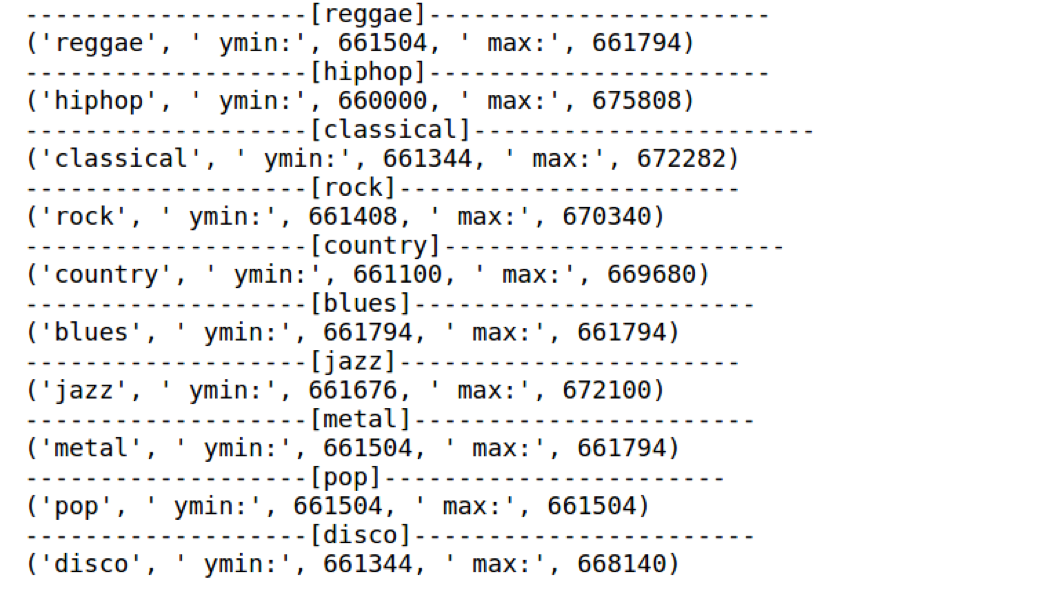
\includegraphics{audiosample.png}
  \caption{Minimum(ymin) and maximum(max) samples for each genre}
  \label{fig:audiosamples}
\end{figure}

\end{center}

\subsubsection{Spectral Rolloff}
The spectral rolloff is defined as the frequency $R_{t}$ below which 85\% of the magnitude distribution is concentrated.
$$ \sum_{n=1}^{R_{t}}M_{t}[n] = 0.85 * \sum_{n=1}^{N}M_{t}[n]. $$
The rolloff is another measure of spectral shape.

\subsubsection{Time Domain Zero Crossings}
$$Z_{t} = \frac{1}{2}\sum_{n=1}^{N}|sign(x[n])-sign(x[n-1])|$$
where the $sign$ function is 1 for positive arguments and 0 for negative arguments and $x[n]$ is the time domain signal for frame $t$. Time domain zero crossings provide a measure of the noisiness of the signal.

\subsubsection{Mel-Frequency Cepstral Coefficients}
Mel-frequency cepstral coefficients (MFCC) are perceptually motivated features that are also based on the STFT. After taking the log-amplitude of the magnitude spectrum, the FFT bins are grouped and smoothed according to the perceptually motivated Mel-frequency scaling. Finally, in order to decorrelate the resulting feature vectors a discrete cosine transform is performed. Although typically 13 coefficients are used for speech representation, we have found that the first five coefficients provide the best genre classification performance.

\subsubsection{Root Mean Square Energy}
 Root-mean-square (RMS) energy for each frame is calculated from the audio samples y.  Computing the energy from audio samples is faster as it doesn’t require a STFT calculation.  However, another option is using a spectrogram  which will give a more accurate representation of energy over time because its frames can be windowed.

\subsubsection{Spectral Contrast}
Octave-based Spectral Contrast considers the spectral peak, spectral valley and their difference in each sub-band. For most music, the strong spectral peaks roughly correspond with harmonic components; while non-harmonic components, or noises, often appear at spectral valleys. Thus, Spectral Contrast feature could roughly reflect the relative distribution of the harmonic and non-harmonic components in the spectrum. 

\subsection{Timbral Texture Feature Vector}
To summarize, the feature vector for describing timbral texture consists of the following features: means and variances of spectral centroid, rolloff, zerocrossings over the texture window , rms energy, spectral contrast, and means and variances of the first five MFCC coefficients over the texture window (excluding the coefficient corresponding to the DC component) resulting in a 20-dimensional feature vector.


\subsection{Librosa}
The features were extracted using the python package LibROSA  \cite{brian_mcfee-proc-scipy-2015}. LibROSA is a python package for music and audio analysis. It provides the building blocks necessary to create music information retrieval systems.

\section{Approaches using in-built libraries}
Once the feature extraction is done and we have the dataframe, we can apply standard off the shelf python libraries for classification.

\begin{figure}[ht]
    \centering
    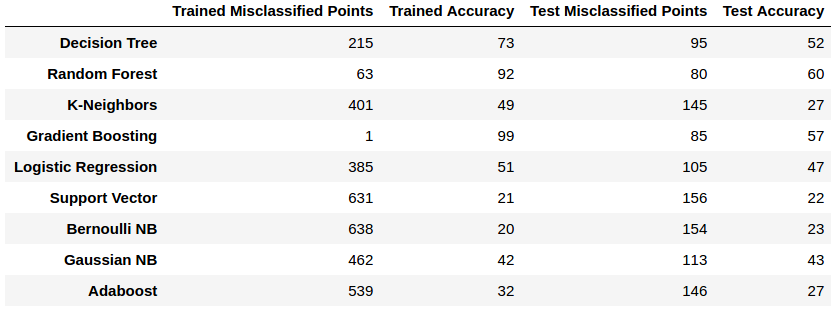
\includegraphics[scale=0.5]{libraryFunctionsTable.png}
    \caption{Off the shelf library functions}
    \label{fig:libraryFunctionsTable}
\end{figure}


From Figure \ref{fig:libraryFunctionsTable} we can see that the best accuracy achieved so far on test dataset is by \textbf{Gradient Boosting}.

\section{Approaches using our implementations}
The dataset is split into 80:20 ratio between training dataset and test dataset randomly. The dataset then remains fixed for all training models.

In this section, we will explain about the model which we implemented.

\subsection{Multi-class Neural Network1}
The neural network which we implemented had following configuration:
\begin{itemize}
 \item \textbf{Hidden Layers}: 7
 \item \textbf{Neurons per hidden layer}: 40
 \item \textbf{Learning Rate}: 0.01
 \item \textbf{Iterations}: 10,000
\end{itemize}

\begin{table}[ht]
    \centering
    \caption{Neural Network Accuracy}
    \label{tbl:neural-network-accuracy}
    \begin{tabular}{|l|r|r|}
    \hline
                   & \textbf{Misclassified} & \textbf{Accuracy} \\ \hline
    \textbf{Train} & 10                     & 98.0\%            \\ \hline
    \textbf{Test}  & 112                    & 44.0\%            \\ \hline
    \end{tabular}
\end{table}

From Table \ref{tbl:neural-network-accuracy}, we can see that our multi-class neural network outperformed 5 out of 9 in-built library functions (Ref: Figure \ref{fig:libraryFunctionsTable}).

\subsection{Decision Trees}
The configuration of our decision tree is:
\begin{itemize}
 \item \textbf{Maximum depth of tree}: 20
 \item \textbf{Minimum record count}: 2
\end{itemize}

\begin{figure}[ht]
    \centering
    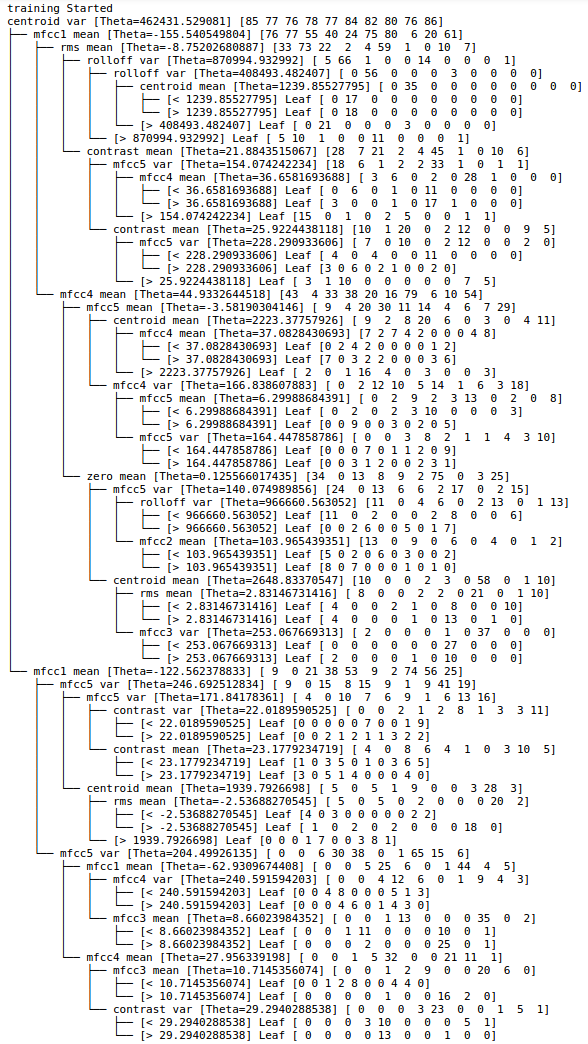
\includegraphics[scale=0.7]{withoutMargin.png}
    \caption{Decision Tree}
    \label{fig:decision_tree}
\end{figure}

\begin{table}[!ht]
    \centering
    \caption{Decision Tree Accuracy}
    \label{tbl:decision-tree-accuracy}
    \begin{tabular}{|l|r|r|}
    \hline
                   & \textbf{Misclassified} & \textbf{Accuracy} \\ \hline
    \textbf{Train} & 0                      & 100.0\%           \\ \hline
    \textbf{Test}  & 100                    & 50.0\%            \\ \hline
    \end{tabular}
\end{table}

From Table \ref{tbl:decision-tree-accuracy}, we can see that our decision tree model outperformed 6 out of 9 in-built library functions (Ref: Figure \ref{fig:libraryFunctionsTable}).

\begin{figure}[!ht]
    \centering
    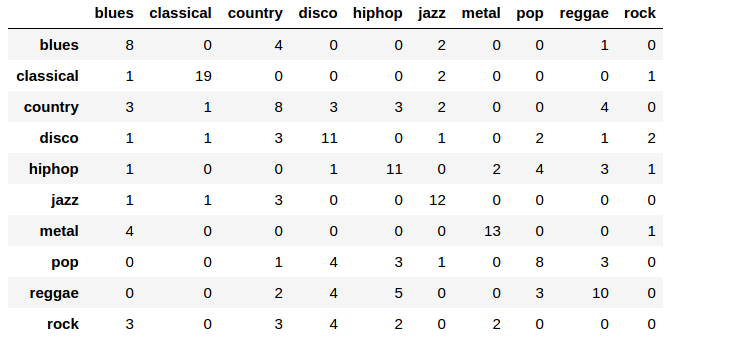
\includegraphics[scale=0.5]{decision_cmtx_testdata.png}
    \caption{Confusion Matrix of Decision Tree}
    \label{fig:dt-cmtx-test}
\end{figure}

Figure \ref{fig:dt-cmtx-test} shows the confusion matrix of test data classification by our Decision Tree model.

You can also see the decision tree in Figure \ref{fig:decision_tree}.

\subsection{Random Forest}
Our Random Forest model is a wrapper around the decision tree model. We randomly partition the dataset into multiple data subsets and train the decision tree on each subset.
The configuration of the Random Forest model is:
\begin{itemize}
 \item \textbf{Number of trees}: 50
  \item \textbf{Maximum depth of tree}: 7
 \item \textbf{Minimum record count}: 20
\end{itemize}

\begin{table}[ht]
    \centering
    \caption{Decision Tree Accuracy}
    \label{tbl:random-forest-accuracy}
    \begin{tabular}{|l|r|r|}
    \hline
                   & \textbf{Misclassified} & \textbf{Accuracy} \\ \hline
    \textbf{Train} & 8                      & 99.0\%            \\ \hline
    \textbf{Test}  & 73                     & 63.5\%            \\ \hline
    \end{tabular}
\end{table}

From Table \ref{tbl:random-forest-accuracy}, we can see that our random forest model outperformed 9 out of 9 in-built library functions (Ref: Figure \ref{fig:libraryFunctionsTable}).

\begin{figure}[ht]
    \centering
    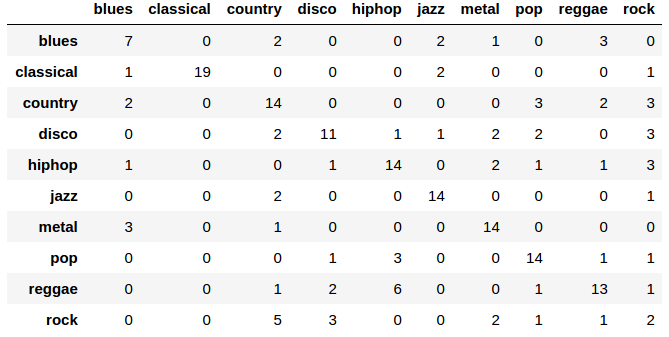
\includegraphics[scale=0.5]{rf_cmtx_test.png}
    \caption{Confusion Matrix of Random Forest}
    \label{fig:rf-cmtx-test}
\end{figure}

Figure \ref{fig:rf-cmtx-test} shows the confusion matrix of test data classification by our Random Forest model.

\subsection{Convolutional Neural Network}
We also made an attempt at classification of genres using the Power Spectrogram of the audio files. We processed the audio files and came up with the spectrograms.

\begin{table}[!ht]
    \centering
    \begin{tabular}{ccc}
        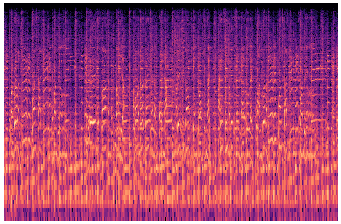
\includegraphics[scale=0.3]{blues.png} &  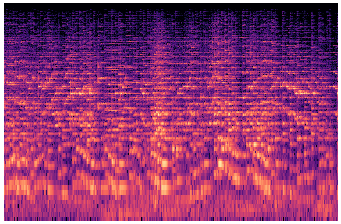
\includegraphics[scale=0.3]{classical.png} & 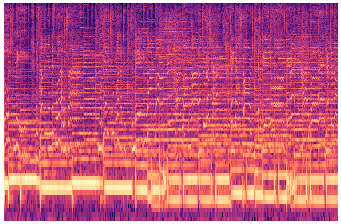
\includegraphics[scale=0.3]{country.png}\\ 
        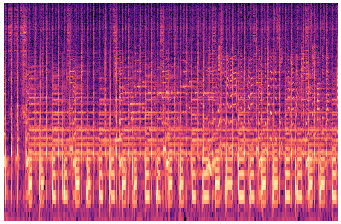
\includegraphics[scale=0.3]{disco.png} &  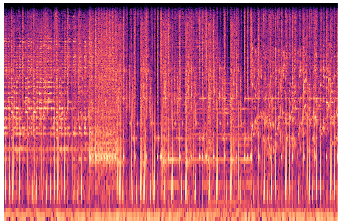
\includegraphics[scale=0.3]{hiphop.png} & 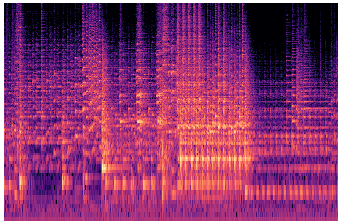
\includegraphics[scale=0.3]{jazz.png}\\ 
        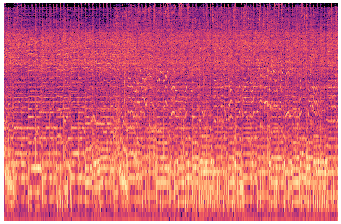
\includegraphics[scale=0.3]{metal.png} &  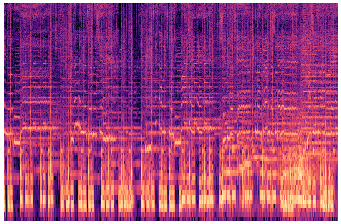
\includegraphics[scale=0.3]{pop.png} & 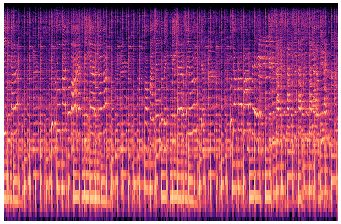
\includegraphics[scale=0.3]{reggae.png}\\ 
    \end{tabular}
    \caption{Power Spectrograms of Blues, Classical, Country, Disco, Hiphop, Jazz, Metal, Pop and Reggae}
    \label{tab:spectrograms}
\end{table}

From Table \ref{tab:spectrograms} we can see that the spectrograms are quite distinct from each other. Each genre has a particular rhythm which is captured in this image. We tried to classify the genres by training a Convolutional neural network on these images.

We used tensorflow library for creating the model. Since the data set is very small, the accuracy achieved by our model is very poor. The model is as follows:
\begin{itemize}
    \item Image size is 200 x 200 x 4
    \item 2 pairs of Convolutional and Max Pooling Layers
    \item A fully connected hidden layer of size 128
    \item A fully connected output layer of size 10
    \item Batch Gradient Descent learning rate is $1e^{-4}$ and batch size of 50
\end{itemize}

The accuracy on test data is \textbf{0.228924}.

\section{Observations and Conclusions}
The original paper \cite{GTZAN} achieved the accuracy of 61\% using Timbral Features as well as Rhythmic Features of the audio files.

We were able to achieve more accuracy (63.5 \%) than them using only Timbral Features.

Also we were able to achieve much better accuracy than most standard library implementations of classification algorithms.

\section{Future Work}
Since we are only using Timbral features and still able to achieve a good accuracy, we believe that if we also include Rhythmic features in our dataset, we may be able to achieve much higher accuracy then what we are getting now.

Also the dataset which we used in this project was very small (only 1000 audio files) and not sufficient to train a neural network. We can train our models on a much bigger dataset available openly at \cite{Bertin-Mahieux2011}.

\section{Timeline}
\subsection{Before Mid Stage Presentation}
\begin{itemize}
 \item Analysis of spectrum of audio files
 \item Using standard neural network library implementation for classification
\end{itemize}
\subsection{After Mid Stage Presentation}
\begin{itemize}
 \item Setting up audio processing libraries
 \item Pre-processing of audio files
 \item Classification using standard off-the-shelf libraries
 \item Building our own models
 \begin{itemize}
  \item Multi-Class Neural Network
  \item Decision Tree
  \item Random Forest
  \item Convolutional Neural Network
 \end{itemize}
\end{itemize}

\section{Contributions}
\begin{itemize}
\item \textbf{Abhijeet Dubey}: Preprocessing, spectral analysis
 \item \textbf{Anshul Gupta}: Convolutional Neural Network, Standard Libraries (KNN, Multinomial Naive Bayesian, Logistic Regression, SVC, Random Forest, etc.)
 \item \textbf{Khursheed Ali}: Decision Trees, Random Forest
 \item \textbf{Nithin S}: Multi-Class Neural Networks
 
\end{itemize}
Feature extraction: Done by everyone.

\bibliographystyle{unsrt}
\bibliography{References}


\end{document}